\documentclass{article}

\usepackage{geometry}
\usepackage{gbt7714}
\usepackage{xeCJK}
\usepackage{booktabs}       % professional-quality tables
\usepackage{amsfonts}       % blackboard math symbols
\usepackage{subfig}
\usepackage{amsmath}
\usepackage{graphicx}
\usepackage{float}
\usepackage{svg}

\graphicspath{{assets/}}

\linespread{1.5}
\geometry{a4paper, left=2.5cm, right=2.5cm, top=2.5cm, bottom=2.5cm}
\bibliographystyle{gbt7714-numerical}   
\title{Anomaly Sound Detection in High-Voltage Shunt Reactors Based on Soft-Constrained Latent Regularized Adversarial Learning}

\begin{document}
\maketitle

\begin{abstract}
  This paper proposes a soft-constrained latent regularized adversarial anomaly detection method (Soft-LRAAD) to address the problem of hard constraints on the upper bound of the KL divergence of the spectrogram generated by the generator due to the hyperparameter M in the LRAAD method. The LRAAD method uses hard constraints to control the upper bound of the KL divergence, which not only makes it difficult for the model to effectively separate normal and anomalous data in latent space but also causes instability during model training, ultimately affecting model performance.
  To solve this problem, the Soft-LRAAD method introduces a soft constraint loss to replace the hard constraint loss, using a smooth function to approximate the upper bound constraint loss of the KL divergence. This approach improves the model's ability to distinguish between normal and anomalous data in latent space, enhances the stability of model training, and thus improves overall performance.
  Experiments conducted on sound datasets measured at substations demonstrate that the Soft-LRAAD method achieves significantly better AUC scores in anomaly detection tasks than other baseline models, validating the effectiveness and practicality of the proposed method. This method provides a new solution for anomaly sound detection in the state monitoring of high-voltage reactors.
\end{abstract}

Keywords: Acoustic Anomaly Detection, Semi-Supervised Learning, Adversarial Learning, Latent Variable Regularized Adversarial Learning

\section{Introduction}

High-voltage shunt reactors play a crucial role in ultra-high voltage (UHV) substations, primarily functioning to compensate reactive power, stabilize grid voltage, and prevent overvoltage in the power system \cite{das2017novel, magdaleno2014temperature, tumay2017review}. Due to the complex operating environment of UHV substations, high-voltage shunt reactors may experience various faults during long-term operation, such as arc discharge, winding loosening, mechanical vibration, etc. \cite{yao2015noninvasive, velasquez2019root}. These faults are often accompanied by abnormal sound signals, making anomaly sound detection in high-voltage shunt reactors critical for ensuring the safety and reliability of the power system.

Currently, the main methods for anomaly detection in high-voltage shunt reactors include oil chromatography detection, ultrasonic partial discharge detection, and high-frequency partial discharge detection. Although these methods can help identify potential internal faults to some extent, they also have limitations:

\begin{enumerate}

  \item{\textbf{Oil Chromatography Detection:} Oil chromatography is a mature fault diagnosis method that mainly detects discharge or overheating issues by analyzing the gas components in the oil \cite{ali2023conventional}. Although oil chromatography can provide early warning information on discharge or overheating faults, its detection cycle is long, lacks real-time capability, and struggles to reflect the instantaneous state changes of the reactor. Furthermore, its sensitivity to early and minor faults is low, which may lead to faults being detected only at a more severe stage.}

  \item{\textbf{Ultrasonic and High-Frequency Partial Discharge Detection:} Ultrasonic detection captures ultrasonic signals generated by partial discharge within the reactor \cite{wang2018partial}, while high-frequency detection uses high-frequency electromagnetic wave signals to detect partial discharge phenomena within the reactor \cite{zheng2020feasibility}. These methods have high sensitivity in detecting partial discharge in high-voltage equipment, especially in diagnosing insulation aging or partial discharge inside the equipment. However, the accuracy and sensitivity of these methods are easily affected by environmental noise and external interference, particularly in complex electromagnetic environments where detection results may be unstable. Moreover, ultrasonic and high-frequency partial discharge detection methods are limited in detecting mechanical faults and vibration issues in equipment, making it difficult to comprehensively reflect the operational state of high-voltage shunt reactors.}

\end{enumerate}

In contrast, acoustic signal-based detection methods can monitor both mechanical and electrical faults during equipment operation without being limited by oil quality changes and partial discharge signals, offering better real-time performance and robustness \cite{ilkhechi2021applications, gao2022early}. The Soft-LRAAD method proposed in this paper leverages soft-constrained latent regularization adversarial anomaly detection technology, combined with the advantages of deep learning models in acoustic signal analysis, to effectively improve the accuracy and reliability of fault detection in high-voltage shunt reactors.

With the rapid development of artificial intelligence technology, data-driven anomaly detection methods have become a research hotspot. In recent years, deep learning technology has made significant progress in image recognition, speech processing, and other fields, providing new ideas for anomaly detection in high-voltage shunt reactors. Specifically, the combination of adversarial learning and latent variable models allows for the effective extraction of deep features from data, enabling high-precision identification of anomalous patterns. However, existing adversarial learning methods, such as Latent Regularized Adversarial Anomaly Detection (LRAAD), still face some challenges when applied to anomaly detection in high-voltage shunt reactors. The LRAAD method uses hard constraints to control the upper bound of KL divergence in latent space, which, although it helps distinguish between normal and anomalous data, can lead to instability during training, affecting the final detection performance. Additionally, the introduction of hard constraints may result in insufficient flexibility in the latent space, making it difficult to capture the diversity and complexity of anomalous data.

To address these issues, this paper proposes a soft-constrained latent regularized adversarial anomaly detection method (Soft-LRAAD) for anomaly detection in high-voltage shunt reactors. By introducing a soft constraint loss function to replace the hard constraint loss in the LRAAD method, this approach more flexibly handles the distribution of normal and anomalous data in latent space. This improvement not only enhances the stability of model training but also boosts the model's anomaly detection performance under various conditions. Furthermore, experiments on sound datasets measured at UHV substations demonstrate that the proposed Soft-LRAAD method outperforms traditional methods in anomaly detection tasks, providing superior performance.

The main contributions of this paper include:

\begin{enumerate}

  \item Proposing the Soft-LRAAD anomaly detection method, which controls the upper bound of KL divergence in the generator's spectrogram using soft boundaries, significantly improving the separation of normal and anomalous data in latent space, thereby enhancing the accuracy and robustness of anomaly detection.

  \item Designing an anomaly score based on KL divergence loss and reconstruction loss. Compared to methods that use only reconstruction loss as an anomaly score, the anomaly score based on KL divergence and reconstruction loss can better distinguish between normal and anomalous data, improving anomaly detection performance.

  \item Validating the model using real-world sound data from UHV substations. Experimental results show that the Soft-LRAAD method exhibits high anomaly detection accuracy and robustness under different load conditions.

\end{enumerate}

The structure of this paper is as follows: Chapter 2 introduces related research work and background knowledge; Chapter 3 introduces the background of the LRAAD model; Chapter 4 details the design and implementation of the Soft-LRAAD model, including the architecture of the encoder and generator and their training methods; Chapter 5 presents the experimental settings and dataset partitioning, followed by an analysis and discussion of the experimental results; Chapter 6 summarizes the research work and suggests future research directions.

\section{Related Work}

Previous research has covered a variety of acoustic anomaly detection methods and related technologies. Some methods rely on traditional signal processing techniques, while others utilize emerging technologies such as deep learning and artificial intelligence \cite{mnasri2022anomalous, jombo2023acoustic}. Traditional signal processing-based methods typically involve feature extraction, pattern recognition, and classification. These methods often include techniques such as filtering, time-frequency analysis, and spectral analysis to extract features from sound signals and use classifiers (e.g., Support Vector Machine, k-Nearest Neighbors) to identify anomalies. Although traditional methods have achieved certain successes in some cases, they are limited by reliance on manual feature design and parameter adjustment and struggle to handle complex nonlinear relationships and large-scale data \cite{pang2021deep, chalapathy2019deep, shi2021equipment}.

In recent years, with the development of deep learning technology, methods based on latent variable models have made significant progress in the field of acoustic anomaly detection in power equipment \cite{AE-AD, AE-AD-2, CAE-AD, VAE-AD, VAE-AD-2, SAE-AD}. For example, Duman et al. \cite{CAE-AD} proposed an industrial process acoustic anomaly detection method based on Convolutional Autoencoders (CAE), using log-scaled Mel-spectrogram features as input. Compared to traditional anomaly detection methods such as One-Class Support Vector Machine (OCSVM) \cite{ocsvm}, the CAE method demonstrates better anomaly detection performance in industrial processes. Variational Autoencoder (VAE)-based anomaly detection methods \cite{VAE-AD, VAE-AD-2} introduce latent variables and KL divergence to learn latent representations of data, enhancing the model's generalization ability. For example, An et al. \cite{VAE-AD} proposed a VAE-based anomaly detection method that trains a VAE model to learn latent representations of normal data and uses KL divergence to measure the difference between normal and anomalous data.

% In recent years, the student-teacher method has also gained widespread attention in anomaly detection. Zhang et al. \cite{destseg} proposed the DeSTSeg model, including a pre-trained teacher network, a denoising student network, and a segmentation network. The model is trained in two steps. First, the synthetic anomaly images are used as inputs to the student network, and the original clean images are used as inputs to the teacher network. The parameters of the segmentation network are optimized to locate the anomaly regions. Then, during inference, pixel-level anomaly maps are generated through post-processing, and image-level anomaly scores are calculated. Batzner et al. \cite{efficientad} proposed the EfficientAD method, which uses a pre-trained neural network to extract features from images and uses a lightweight student-teacher model to detect anomaly features during testing. The paper also introduced a novel loss function for training the student-teacher model.

GAN-based anomaly detection methods have made significant progress in the field of image anomaly detection. The literature \cite{anogan} proposes a GAN-based anomaly detection method that models normal samples to identify anomalies. f-AnoGAN \cite{f-anogan} is an improvement of the AnoGAN method \cite{anogan}. While AnoGAN uses an iterative method to find the latent space representation of an image, f-AnoGAN learns a mapping from the image to the latent space, significantly improving speed. The literature \cite{ganomaly} proposes a new encoder-decoder-encoder architecture model called GANomaly, which uses reconstruction loss, latent representation loss, and adversarial loss to train the model and calculate anomaly scores. The experiments show that its performance is superior to state-of-the-art GAN-based and traditional autoencoder-based anomaly detection methods, with the ability to generalize to any anomaly detection task. Jiang et al. \cite{AEGAN-AD} proposed an unsupervised model AEGAN-AD for machine audio anomaly detection using GANs. The research shows that by introducing a discriminator to provide feature-level guidance, the AEGAN-AD model can better understand representations rather than just focusing on surface noise, addressing the issue that CAE may reconstruct anomaly signals and WaveNet's long training and prediction time. The experimental results show that the AEGAN-AD model achieved outstanding performance in the DCASE 2022 challenge, reaching state-of-the-art performance levels.

The LRAAD model combines the advantages of adversarial learning and latent variable models, enabling the effective extraction of deep features from data and the high-precision identification of anomalous patterns. However, the introduction of hard constraints in the LRAAD method can lead to instability during model training, affecting the final detection performance. To address this issue, this paper proposes a soft-constrained latent regularized adversarial anomaly detection method (Soft-LRAAD) for anomaly detection in high-voltage shunt reactors. The Soft-LRAAD method replaces hard constraints with soft constraint losses, improving the model's ability to distinguish between normal and anomalous data in latent space, enhancing training stability, and ultimately improving overall performance.

\section{Background}

\textbf{Evidence Lower Bound:} The Evidence Lower Bound (ELBO) is a crucial concept in Variational Autoencoder (VAE) used to measure the difference between the distribution of latent variables and the true distribution. ELBO consists of two parts: the reconstruction error, which measures the difference between the data generated by the generator and the original data, and the KL divergence, which measures the difference between the distribution of latent variables and the prior distribution. By maximizing the ELBO, the generated data can be made closer to the real data, and the distribution of latent variables can be made closer to the prior distribution. The formula for the ELBO is as follows:

\begin{equation}
  ELBO(x)=\mathbb{E}_{q_{\phi}(z \mid x)}[\log p_{\theta}(x \mid z)]-D_{\mathrm{KL}}\left(q_{\phi}(z \mid x) \| p(z)\right) 
\end{equation}

\textbf{LRAAD:} Latent Regularized Adversarial Anomaly Detection (LRAAD) is an anomaly detection method based on adversarial learning, using an encoder and generator to learn latent representations of normal data and using adversarial learning to distinguish between normal and anomalous data. The core idea of the LRAAD model is to minimize the KL divergence between the latent representations of normal data and the standard normal distribution, mapping normal data to a normal distribution in latent space while mapping anomalous data to a non-normal distribution in latent space. This allows the LRAAD model to better distinguish between normal and anomalous data, achieving anomaly detection.

\begin{figure}[H]
    \centering
    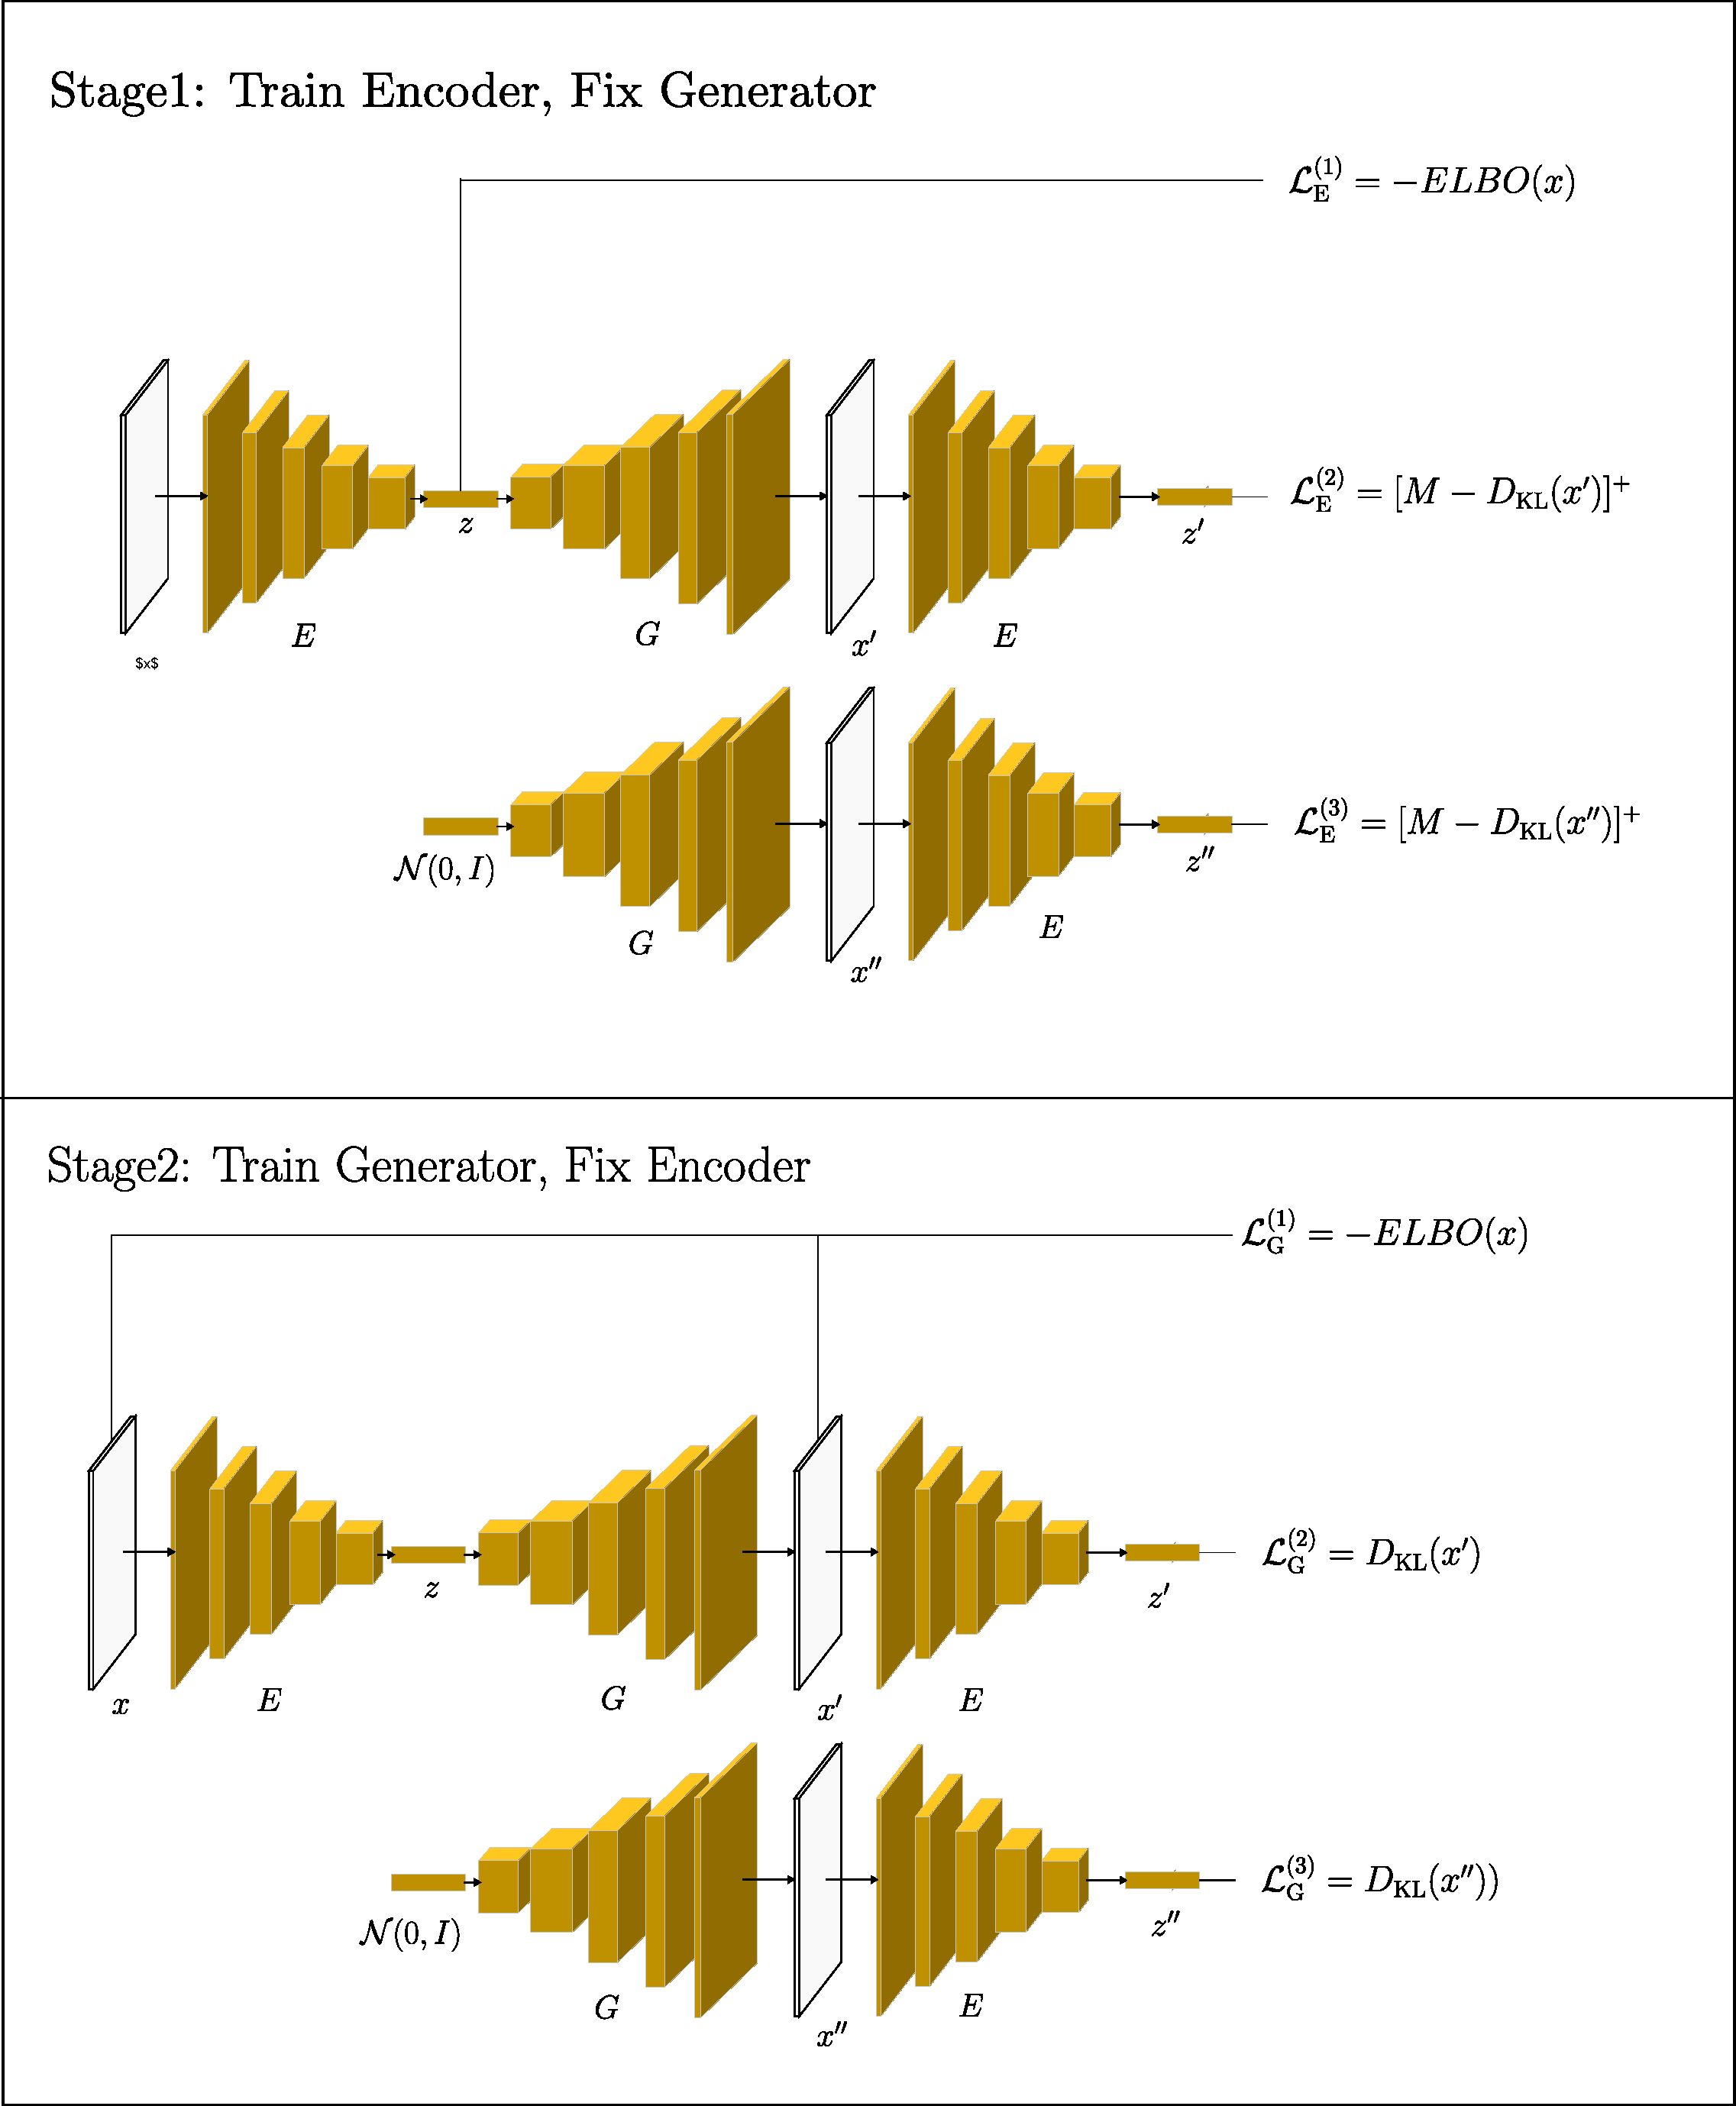
\includegraphics[width=\textwidth]{./assets/lraad.pdf}
    \caption{The Training Pipeline of LRAAD}
    \label{fig:lraad}
\end{figure}

\begin{figure}[H]
    \centering
    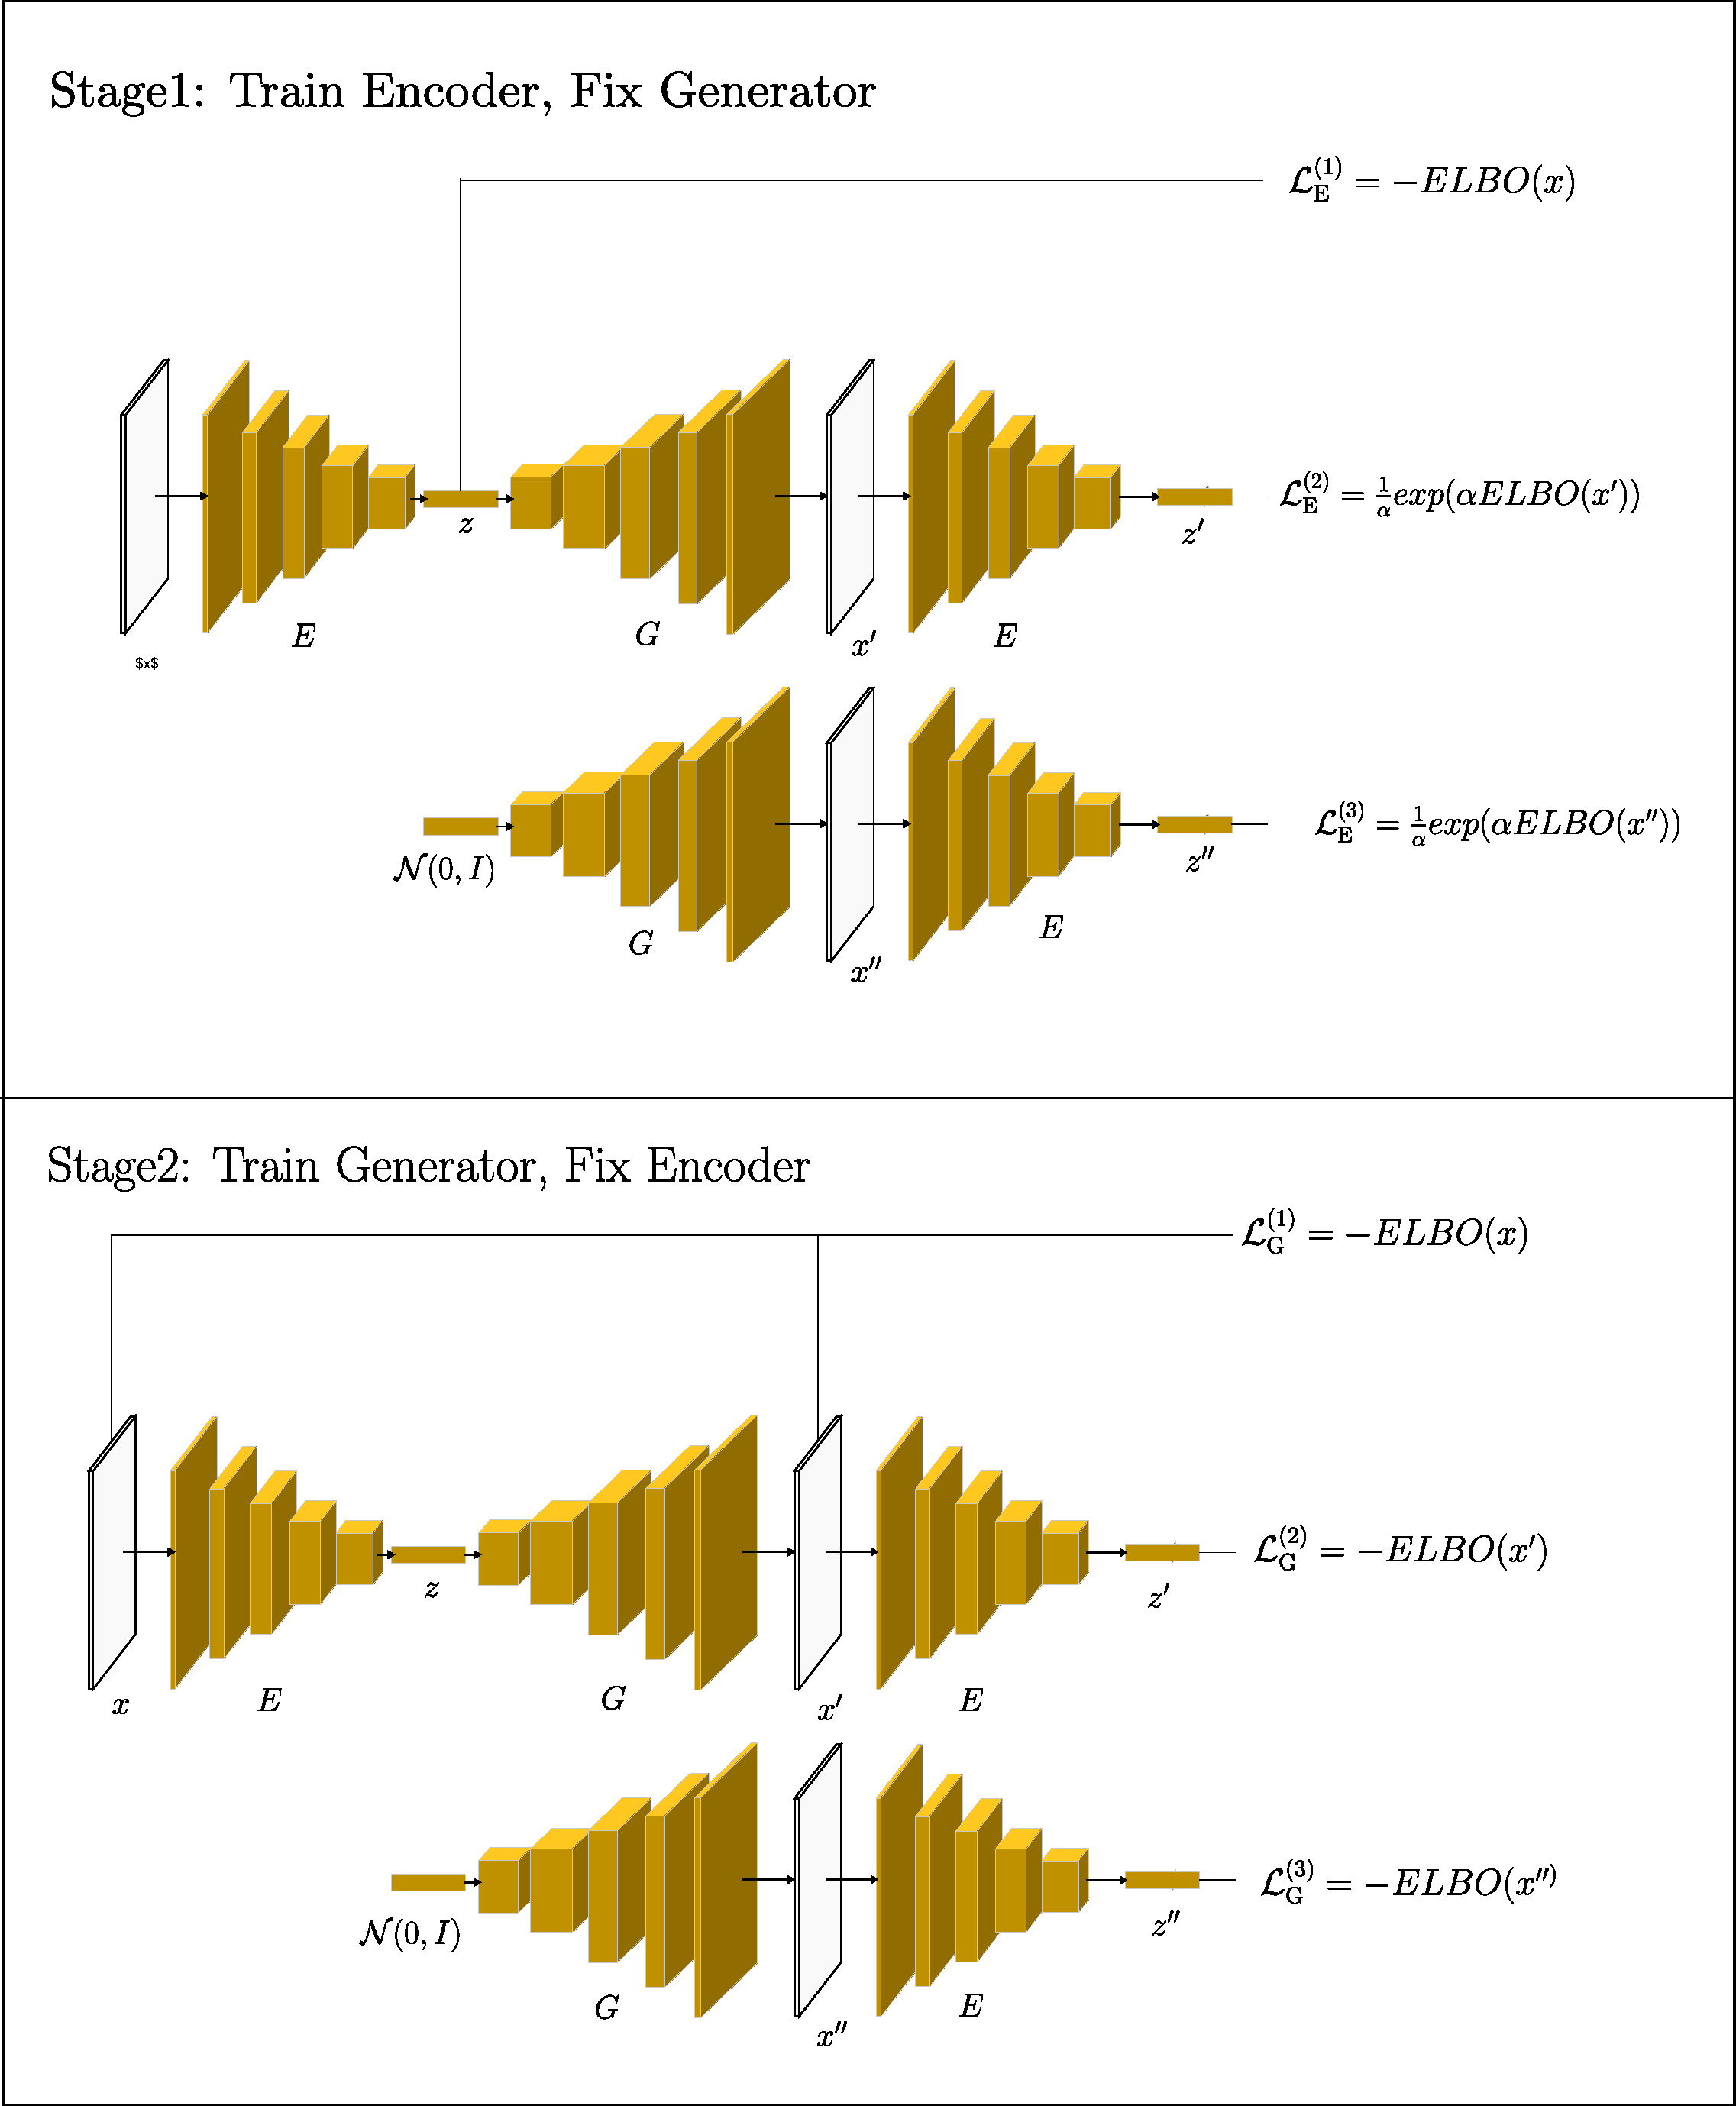
\includegraphics[width=\textwidth]{./assets/soft_lraad_model.pdf}
    \caption{The Training Pipeline of Soft-LRAAD}
    \label{fig:soft_lraad}
\end{figure}

Let $D_{\mathrm{KL}}(x) = D_{\mathrm{KL}}(q(\cdot \mid x) \| p(\cdot))$. Here, $q(\cdot \mid x)$ represents the distribution of the latent representation of the spectrogram $x$ encoded by the encoder, $p(\cdot)$ represents the standard normal distribution, denoted as $\mathcal{N}(0, I)$, and $D_{\mathrm{KL}}$ represents the KL divergence.

\begin{equation}
  \mathcal{L}_{\mathrm{E}}=\left\|x-x^{\prime}\right\|^2 + D_{\mathrm{KL}}(x) + [M - D_{\mathrm{KL}}(x^\prime)]^{+} + [M - D_{\mathrm{KL}}(x^{\prime\prime})]^{+}
\end{equation}

\begin{equation}
  \mathcal{L}_{\text {G}}= \left\|x-x^{\prime}\right\|^2 + D_\mathrm{KL}(x^\prime) + D_\mathrm{KL}(x^{\prime\prime})
\end{equation}

Equivalently,

\begin{equation}
  \mathcal{L}_{\mathrm{E}}=-ELBO(x) + [M - D_{\mathrm{KL}}(x^\prime)]^{+} + [M - D_{\mathrm{KL}}(x^{\prime\prime})]^{+}
\end{equation}

\begin{equation}
  \mathcal{L}_{\text {G}}=-ELBO(x) + D_\mathrm{KL}(x^\prime) + D_\mathrm{KL}(x^{\prime\prime})
\end{equation}

Here, $[M - D_{\mathrm{KL}}]^{+}$ represents the KL divergence constraint term for the generated images, defined as $max(0, M - D_{\mathrm{KL}})$, where $M$ is a hyperparameter used to control the upper bound of KL divergence and prevent the KL divergence of the generated images from becoming infinite.

\section{Soft-LRAAD}

\subsection{Overview of the Soft-LRAAD Method}

Soft-LRAAD (Soft-Constrained Latent Regularization Adversarial Anomaly Detection) is an improved anomaly detection method designed to overcome the limitations of the LRAAD method, which suffers from insufficient separation capability in latent space and instability during model training due to hard constraints. By introducing a soft constraint loss function, Soft-LRAAD not only effectively distinguishes between normal and anomalous data but also improves the stability of model training.

The LRAAD method uses hard constraints to control the upper bound of the KL divergence of generated images, and the introduction of hard constraints often makes it difficult for the model to distinguish between normal and anomalous data in latent space. Moreover, hard constraints may lead to gradient instability during training, affecting the overall performance of the model. To address these issues, the Soft-LRAAD method proposes using a soft constraint loss function to replace the hard constraint loss.

In the Soft-LRAAD method, we use a smooth function $\frac{1}{\alpha}exp(- \alpha D_{\mathrm{KL}}(x))$ to approximate the upper bound constraint loss $[M - D_{\mathrm{KL}}(x)]^{+}$ of the KL divergence. The function graphs are shown in Figures \ref{fig:hard_constraints} and \ref{fig:soft_constraints}. Specifically, we replace the hard constraint loss in LRAAD with a soft constraint loss function $\frac{1}{\alpha}exp(- \alpha D_{\mathrm{KL}}(x^\prime)) + \frac{1}{\alpha}exp(-\alpha D_{\mathrm{KL}}(x^{\prime\prime}))$. The introduction of hard constraints sets strict boundaries in latent space, limiting the KL divergence of generated images below the boundary $M$, thereby limiting the model's performance. In contrast, the soft constraint approximates the upper bound of the KL divergence using a smooth function, alleviating this limitation. This allows the model to better separate normal and anomalous data in latent space while maintaining the quality of the generated images.

\begin{figure}[H]
  \begin{minipage}{0.45\textwidth}
    \centering
    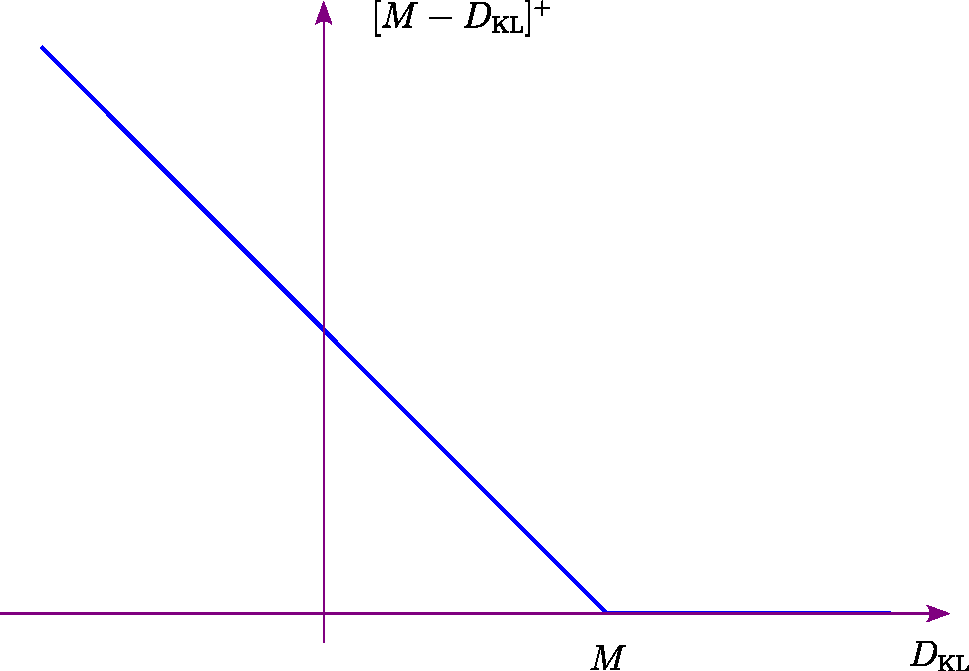
\includegraphics[width=\textwidth]{./assets/hard_constraints.pdf}
    \caption{The hard constraints function $[M - D_{\mathrm{KL}}]^{+}$ of KL divergence in LRAAD}
    \label{fig:hard_constraints}
  \end{minipage}
  \hfill
  \begin{minipage}{0.45\textwidth}
    \centering
    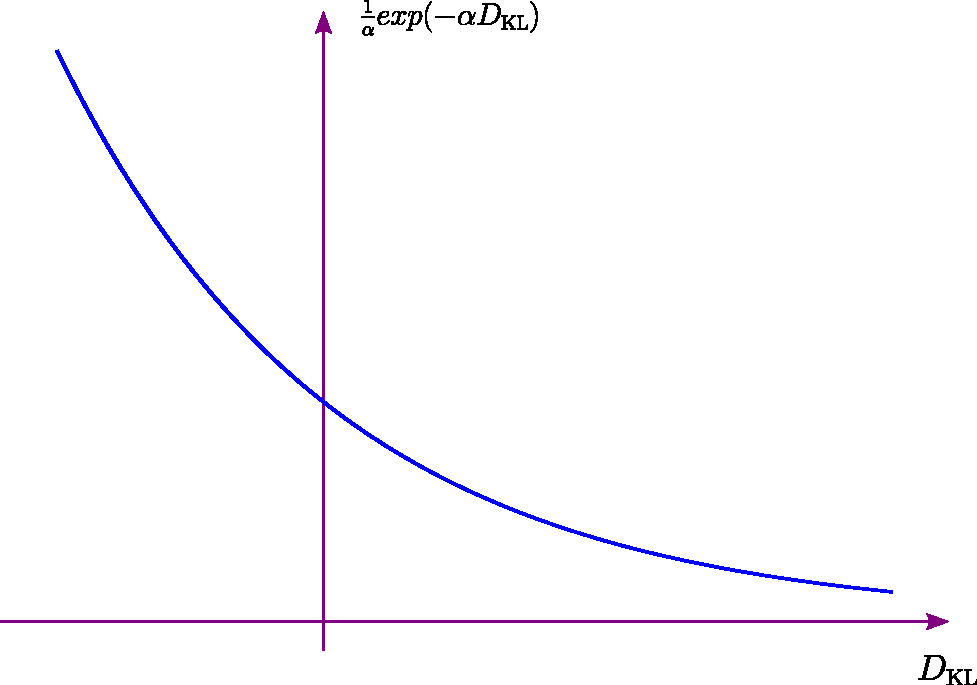
\includegraphics[width=\textwidth]{./assets/soft_constraints.pdf}
    \caption{The soft constraints function $\frac{1}{\alpha}exp(- \alpha D_{\mathrm{KL}})$ of KL divergence in Soft-LRAAD}
    \label{fig:soft_constraints}
  \end{minipage}
\end{figure}

\subsection{Soft Constraint Loss}

The soft constraint loss in the Soft-LRAAD method is one of the key improvements over the LRAAD method. The LRAAD method uses hard constraints to control the upper bound of the KL divergence of generated images, leading to difficulties in effectively distinguishing between normal and anomalous data in latent space, as well as potential instability during training. To overcome these challenges, Soft-LRAAD introduces a soft constraint loss that uses a smooth function to approximate the upper bound constraint loss of the KL divergence, alleviating the issues caused by hard constraints.

To overcome the shortcomings of hard constraints, the Soft-LRAAD method introduces a soft constraint loss. The soft constraint loss function is of the form $\frac{1}{\alpha}\exp(- \alpha D_{\mathrm{KL}}(x))$, where $\alpha$ is a tunable hyperparameter. Compared to hard constraints, the function graph of the soft constraint shows a smooth decreasing trend. This design allows the loss to decrease gradually even when the KL divergence approaches the threshold, rather than remaining constant as in the case of hard constraints, allowing the KL divergence of the generated images to increase without becoming infinite. In this way, the Soft-LRAAD method better maintains the quality of generated images while improving the model's anomaly detection performance.

Unlike the LRAAD method, Soft-LRAAD adopts a soft-constrained approach to handle the KL divergence term, making the model more flexible in penalizing the KL divergence during training. Specifically, the encoder loss function $\mathcal{L}_{\mathrm{E}}$ and generator loss function $\mathcal{L}_{\mathrm{D}}$ of Soft-LRAAD are defined as follows:

\begin{equation}
  \mathcal{L}_{\mathrm{E}}=-ELBO(x) + \frac{1}{\alpha}exp(- \alpha D_{\mathrm{KL}}(x^\prime)) + \frac{1}{\alpha}exp(-\alpha D_{\mathrm{KL}}(x^{\prime\prime}))
\end{equation}

\begin{equation}
  \mathcal{L}_{\text {G}}=-ELBO(x) + D_\mathrm{KL}(x^\prime) + D_\mathrm{KL}(x^{\prime\prime})
\end{equation}

where $\alpha$ is a tunable hyperparameter used to control the influence of the soft constraint term.

For the KL divergence term, an additional reconstruction loss term is added to better maintain the quality of generated images while improving the model's anomaly detection performance. In this way, the Soft-LRAAD method better distinguishes between normal and anomalous data, improving the accuracy and robustness of anomaly detection. The corresponding formulas are as follows:

\begin{equation} \label{eq:encoder_loss}
  \mathcal{L}_{\mathrm{E}}=-ELBO(x) + \frac{1}{\alpha}exp(\alpha ELBO(x^\prime)) + \frac{1}{\alpha}exp(\alpha ELBO(x^{\prime\prime}))
\end{equation}

\begin{equation} \label{eq:decoder_loss}
  \mathcal{L}_{\text {G}}=-ELBO(x) - ELBO(x^\prime) - ELBO(x^{\prime\prime})
\end{equation}

The impact of soft constraints on model training is mainly reflected in several aspects. First, soft constraints allow latent variables to be more flexibly distributed in latent space, enhancing the ability to distinguish between normal and anomalous data. Second, the introduction of soft constraints helps stabilize model training, avoiding the gradient discontinuity and instability issues that may arise from hard constraints. Finally, by adjusting the $\alpha$ parameter, the penalization of KL divergence by soft constraints can be flexibly controlled, further optimizing model performance.

\subsection{Model Training}

The structure of Soft-LRAAD is similar to LRAAD, consisting of an encoder $E$ and a generator $G$. The encoder $E$ is responsible for mapping the input Mel-spectrogram $x$ to latent space, while the generator $G$ maps the latent variables back to the Mel-spectrogram domain, achieving spectrogram reconstruction. The overall architecture of Soft-LRAAD is shown in Figure \ref{fig:soft_lraad}.

The training process of Soft-LRAAD mainly includes training the encoder $E$ and the generator $G$. The specific training algorithm is shown in Algorithm 1. The training of Soft-LRAAD is similar to LRAAD, where the encoder and generator are trained adversarially by minimizing their respective loss functions to optimize model parameters. By alternately training the encoder and generator, the Soft-LRAAD model's encoder can better distinguish between normal and anomalous data, and the generator can better reconstruct the input spectrogram, thereby improving anomaly detection accuracy and robustness.

\begin{table}[H]
    \centering
    \begin{tabular}{l}
        \toprule
        \label{tab:training}
        {\textbf{Algorithm 1} Training Soft-LRAAD model} \\
        \midrule
        1: Initialize network parameters \\
        2: \quad {\textbf{For} number of epochs \textbf{do}} \\
        3: \quad\quad Random mini-batch $X$ from dataset \\
        4: \quad\quad Compute latent representation of $X$: $Z = E(X)$ \\
        5: \quad\quad Sample $Z_p$ from prior distribution $p(z)=\mathcal{N}(0, I)$ \\
        6: \quad\quad Compute reconstructed spectrogram of $Z$ and $Z_p$: $X^\prime = G(Z)$, $X^{\prime\prime} = G(Z_p)$ \\
        7: \quad\quad Compute latent representation of $X^\prime$ and $X^{\prime\prime}$: $Z^\prime = E(X^\prime)$, $Z^{\prime\prime} = E(X^{\prime\prime})$ \\
        8: \quad\quad Compute Encoder loss $\mathcal{L}_E$ according to Eq. \ref{eq:encoder_loss} \\
        9: \quad\quad Update Encoder parameters by minimizing $\mathcal{L}_E$ \\
        10: \quad\quad Compute Generator loss $\mathcal{L}_G$ according to Eq. \ref{eq:decoder_loss} \\
        11: \quad\quad Update Generator parameters by minimizing $\mathcal{L}_G$ \\
        12: \quad {\textbf{End For}} \\
        \bottomrule
    \end{tabular}
\end{table}

\subsection{Anomaly Detection}

We adopt the sum of reconstruction error and KL divergence as the anomaly score. The reconstruction error measures the difference between the generated spectrogram and the original input spectrogram, while the KL divergence measures the difference between the latent representation and the standard normal distribution. For normal data, the reconstruction error is small, and the latent representation is close to the standard normal distribution; for anomalous data, the reconstruction error is large, and the latent representation is far from the standard normal distribution. By combining these two metrics, the model can more accurately identify anomalous data. The mathematical expression for the anomaly score is as follows:

\begin{equation}
\mathcal{A}(x)=\|x-G(E(x))\|^2+D_{\mathrm{KL}}(E(x) \| \mathcal{N}(0, I))
\end{equation}

where $\mathcal{A}(x)$ represents the anomaly score of the input spectrogram $x$, $E(x)$ represents the latent representation of the input spectrogram $x$, $G(E(x))$ represents the reconstructed spectrogram of the latent representation $E(x)$, and $D_{\mathrm{KL}}(E(x) \| \mathcal{N}(0, I))$ represents the KL divergence between the latent representation $E(x)$ and the standard normal distribution. By calculating the anomaly score, we can perform anomaly detection on the input spectrogram $x$ to determine whether it is anomalous data.

\section{Experiments}
This section introduces the experimental settings and results. We first introduce the dataset and preprocessing methods used in the experiments, then describe the experimental settings and evaluation metrics in detail, and finally present and analyze the experimental results.

\subsection{Data Preprocessing}

In this study, systematic and detailed preprocessing of the experimental data was conducted to ensure accurate and reliable results for anomaly detection of high-voltage shunt reactor sound signals. The quality of data preprocessing directly affects the model's training effectiveness and detection performance; therefore, we adopted a series of steps to optimize the processing of sound signal data. The specific steps of data preprocessing are as follows:

The experimental data comes from real-world sound data measured from high-voltage shunt reactors at a UHV substation in China. These sound signals were captured by high-sensitivity sensors installed within the substation, with recordings stored in WAV format, each with a sampling rate of 44.1 kHz and a duration of 10 seconds. Since the original audio files were relatively long and contained information from various conditions, we segmented each recording into multiple audio clips, each 1.36 seconds in length. This segmentation ensures that each clip independently reflects the operational state of the reactor and facilitates subsequent feature extraction and model training.

To better capture the characteristic information in the sound signals, we converted the segmented audio clips into Mel-spectrograms. A Mel-spectrogram is a time-frequency representation that uses the Mel scale on the horizontal axis and represents the power spectrum on the vertical axis, which more closely reflects the frequency characteristics of sound signals according to human auditory perception. Compared to traditional spectrograms, Mel-spectrograms focus more effectively on key frequency bands of sound signals and enhance information in the low-frequency range, making signal features more pronounced.

After generating the Mel-spectrograms, we further processed and analyzed the fine changes in the signals by applying a logarithmic transformation to the Mel-spectrograms. Logarithmic transformation compresses the amplitude dynamic range in the spectrum, reducing the impact of the high-frequency components while highlighting the detail information in the low-frequency signals. This transformation makes the spectral data smoother and more stable, helping the model to better learn the anomalous features in the sound signals.

\subsection{Experimental Settings}

In training the Soft-LRAAD model, we need to set multiple hyperparameters to adjust the model's performance, such as the learning rates of the encoder and generator, the weight coefficients of loss functions (e.g., reconstruction loss, adversarial loss, KL divergence loss), the latent space dimension, the soft constraint coefficient, the number of training iterations, etc. The choice of these hyperparameters significantly impacts the model's training and performance, requiring experimentation and validation to determine the optimal combination. The hyperparameter settings used in the experiments are shown in Table \ref{tab:params}:

\begin{table}
    \centering
    \caption{Soft-LRAAD Model Hyperparameter Settings}
    \label{tab:params}
    \begin{tabular}{lr}
        \toprule
        \textbf{Hyperparameter} & \textbf{Setting} \\
        \midrule
        Latent Space Dimension & 32 \\
        Learning Rate (Encoder) & 0.0002 \\
        Learning Rate (Generator) & 0.0002 \\
        Loss Weight (Reconstruction) & 1 \\
        Loss Weight (Adversarial) & 1 \\
        Loss Weight (KL Divergence) & 1 \\
        Alpha (Soft Constraint Coefficient) & 128$\times $128 \\
        Training Epochs & 100 \\
        Batch Size & 32 \\
        Dataset Split & 80\% Training, 30\% Testing \\
        \bottomrule
    \end{tabular}
\end{table}

\subsection{Evaluation Metrics}

In this study, we used multiple evaluation metrics to quantify and compare the performance of different anomaly detection models, particularly for detecting anomalies in high-voltage shunt reactor sound signals. These evaluation metrics include the Receiver Operating Characteristic (ROC) curve, the Area Under the ROC Curve (AUC) value, and the Partial Area Under the ROC Curve (p-AUC) value. The following is a detailed description of these evaluation metrics.

\textbf{ROC Curve:} The ROC curve is a commonly used tool for evaluating the performance of binary classification models. It plots the True Positive Rate (TPR) against the False Positive Rate (FPR), intuitively showing the model's classification ability at different thresholds. For anomaly detection tasks, the ROC curve reflects the model's ability to balance identifying anomalies (positives) and normal data (negatives). Generally, the closer the ROC curve is to the top left corner (i.e., high TPR and low FPR), the better the model's detection performance. In this experiment, we calculated the TPR and FPR at various thresholds for the anomaly scores generated by different models and plotted the ROC curve to compare the anomaly detection capabilities of the models.

\textbf{AUC (Area Under the Curve) Value:} The AUC value is the area under the ROC curve and serves as a comprehensive indicator of the model's classification performance. AUC values range from 0.5 to 1, where 0.5 indicates that the model's performance is equivalent to random classification, and 1 indicates that the model can perfectly distinguish between normal and anomalous data. The closer the AUC value is to 1, the stronger the model's classification ability in anomaly detection. The AUC metric is widely used in this experiment to compare the overall performance of different anomaly detection models. By calculating the AUC values of different models, we can quantitatively analyze their performance in the task of detecting anomalies in high-voltage shunt reactor sound signals.

\textbf{p-AUC (Partial Area Under the Curve) Value:} The p-AUC value is a refinement of the AUC metric, focusing on the area under the ROC curve where the FPR is less than a specific threshold. In practical applications, we often require that the anomaly detection model has a low FPR. Therefore, the p-AUC value better reflects the model's performance in the low-FPR region, i.e., the model's anomaly detection capability under strict conditions. In this experiment, we calculated the p-AUC values when FPR is less than 0.3, 0.2, and 0.1, respectively. These p-AUC values help us evaluate the model's performance under different FPR requirements, providing a more accurate reflection of the model's detection capability in practical applications.

\subsection{Experimental Results}

This section details the experimental results of the Soft-LRAAD model in the task of anomaly detection in high-voltage shunt reactor sound signals and compares and analyzes it with other traditional models and deep learning models. We focus on the detection accuracy, robustness, and performance under different load conditions. To quantify the performance of each model, this paper uses evaluation metrics such as ROC curves, AUC values, and p-AUC values. The experimental results show that the Soft-LRAAD model exhibits excellent detection performance across multiple experimental datasets.

Figure \ref{fig:roc_curve} shows the ROC curves of the Soft-LRAAD model and other models in anomaly detection tasks. In the experiment, the ROC curve of the Soft-LRAAD model is significantly better than traditional methods and other deep learning models, with the curve overall closer to the top left corner, indicating that it can effectively distinguish between normal and anomalous data at different thresholds. Across six different datasets, the ROC curve of the Soft-LRAAD model consistently outperforms other models, demonstrating higher TPR and lower FPR. This indicates that the Soft-LRAAD model can more accurately identify anomalies and effectively reduce the false alarm rate when detecting anomalous sound signals in reactor operation.

Tables \ref{tab:auc}, \ref{tab:p-auc-03}, \ref{tab:p-auc-02}, and \ref{tab:p-auc-01} present the AUC values and p-AUC values of different models on different datasets. The tables show that the Soft-LRAAD model achieved the highest AUC values in most datasets, indicating its stronger classification ability in anomaly detection tasks. Additionally, the Soft-LRAAD model's p-AUC values for FPR less than 0.3, 0.2, and 0.1 are significantly better than those of other models, indicating its superior performance in the low-FPR region. These results demonstrate that the Soft-LRAAD model has higher detection accuracy and robustness in the task of anomaly detection in high-voltage shunt reactor sound signals and can better distinguish between normal and anomalous data.

\begin{figure}[H]
    \centering
    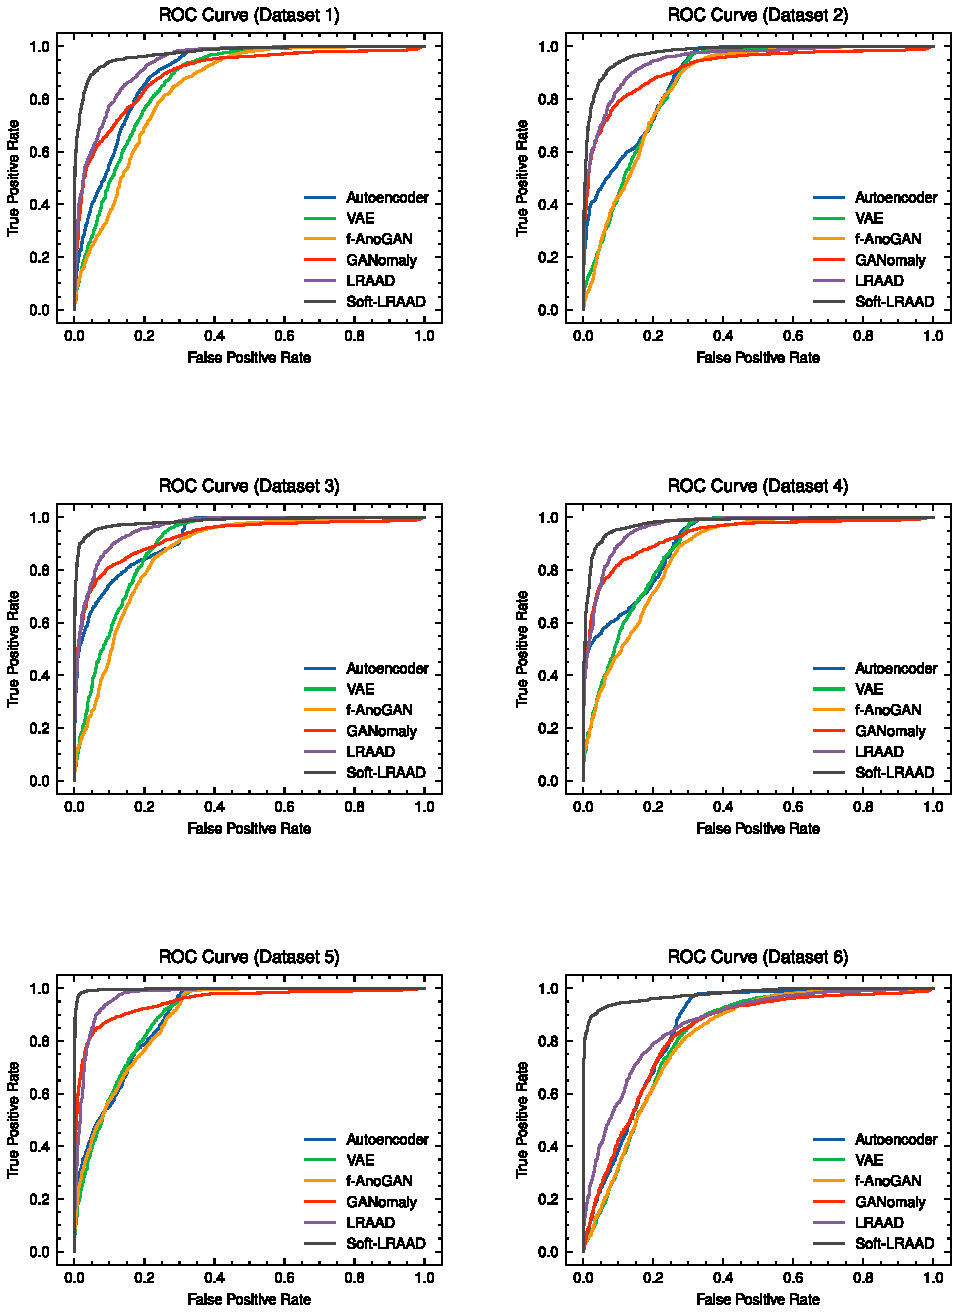
\includegraphics[width=\textwidth]{./roc_curve.pdf}
    \caption{ROC Curves of Different Models on Different Datasets}
    \label{fig:roc_curve}
\end{figure}

\begin{table}[H]
    \centering
    \caption{AUC Comparison of Different Models on Different Datasets}
    \begin{tabular}{ccccccc}
        \toprule
        Dataset & CAE & VAE & f-AnoGAN & GANomaly & LRAAD & Soft-LRAAD(Our) \\
        \midrule
        Dataset1 & 0.8975 & 0.8662 & 0.8400 & 0.8966 & 0.9361 & \textbf{0.9742} \\
        Dataset2 & 0.8911 & 0.8652 & 0.8560 & 0.9195 & 0.9475 & \textbf{0.9755} \\
        Dataset3 & 0.9266 & 0.8958 & 0.8662 & 0.9266 & 0.9607 & \textbf{0.9851} \\
        Dataset4 & 0.9087 & 0.8868 & 0.8654 & 0.9333 & 0.9626 & \textbf{0.9788} \\
        Dataset5 & 0.8962 & 0.8965 & 0.8910 & 0.9511 & 0.9721 & \textbf{0.9975} \\
        Dataset6 & 0.8523 & 0.8178 & 0.8126 & 0.8270 & 0.8674 & \textbf{0.9782} \\
        \bottomrule
    \end{tabular}
    \label{tab:auc}
\end{table}

\begin{table}[H]
    \centering
    \caption{p-AUC Comparison of Different Models on Different Datasets (FPR<0.3)}
    \begin{tabular}{ccccccc}
        \toprule
        Dataset & CAE & VAE & f-AnoGAN & GANomaly & LRAAD & Soft-LRAAD(Our) \\
        \midrule
        Dataset1 & 0.6664 & 0.5824 & 0.5161 & 0.7232 & 0.7930 & \textbf{0.9162} \\
        Dataset2 & 0.6394 & 0.5559 & 0.5487 & 0.7843 & 0.8430 & \textbf{0.9152} \\
        Dataset3 & 0.7605 & 0.6576 & 0.5935 & 0.8076 & 0.8639 & \textbf{0.9538} \\
        Dataset4 & 0.6972 & 0.6252 & 0.5790 & 0.8164 & 0.8342 & \textbf{0.9118} \\
        Dataset5 & 0.6529 & 0.6569 & 0.6423 & 0.8705 & \textbf{0.8866} & 0.8794 \\
        Dataset6 & 0.5262 & 0.4656 & 0.4589 & 0.5243 & 0.6335 & \textbf{0.9377} \\
        \bottomrule
    \end{tabular}
    \label{tab:p-auc-03}
\end{table}

\begin{table}[H]
    \centering
    \caption{p-AUC Comparison of Different Models on Different Datasets (FPR<0.2)}
    \begin{tabular}{ccccccc}
        \toprule
        Dataset & CAE & VAE & f-AnoGAN & GANomaly & LRAAD & Soft-LRAAD(Our) \\
        \midrule
        Dataset1 & 0.5431 & 0.4503 & 0.3809 & 0.6417 & 0.7078 & \textbf{0.8706} \\
        Dataset2 & 0.5355 & 0.4192 & 0.4037 & 0.7324 & 0.7865 & \textbf{0.8798} \\
        Dataset3 & 0.7041 & 0.5225 & 0.4598 & 0.7496 & 0.8176 & \textbf{0.9399} \\
        Dataset4 & 0.6142 & 0.5014 & 0.4532 & 0.7609 & 0.8173 & \textbf{0.9108} \\
        Dataset5 & 0.5465 & 0.5390 & 0.5371 & \textbf{0.8332} & 0.8115 & 0.8306 \\
        Dataset6 & 0.3801 & 0.3190 & 0.3227 & 0.3935 & 0.5377 & \textbf{0.9097} \\
        \bottomrule
    \end{tabular}
    \label{tab:p-auc-02}
\end{table}

\begin{table}[H]
    \centering
    \caption{p-AUC Comparison of Different Models on Different Datasets (FPR<0.1)}
    \begin{tabular}{ccccccc}
        \toprule
        Dataset & CAE & VAE & f-AnoGAN & GANomaly & LRAAD & Soft-LRAAD(Our) \\
        \midrule
        Dataset1 & 0.3640 & 0.2736 & 0.2261 & 0.5268 & 0.5629 & \textbf{0.8279} \\
        Dataset2 & 0.4405 & 0.2472 & 0.2318 & 0.6353 & 0.6658 & \textbf{0.8068} \\
        Dataset3 & 0.6024 & 0.3372 & 0.2651 & 0.6810 & 0.7020 & \textbf{0.9167} \\
        Dataset4 & 0.5487 & 0.3345 & 0.3136 & 0.6635 & 0.6993 & \textbf{0.8059} \\
        Dataset5 & 0.4090 & 0.3700 & 0.3964 & \textbf{0.7626} & 0.7400 & 0.6544 \\
        Dataset6 & 0.2168 & 0.1566 & 0.1624 & 0.2330 & 0.3791 & \textbf{0.8936} \\
        \bottomrule
    \end{tabular}
    \label{tab:p-auc-01}
\end{table}

\section{Conclusion}

In this study, we proposed a soft-constrained latent regularized adversarial anomaly detection method (Soft-LRAAD) for anomaly detection in high-voltage shunt reactor sound signals. The method aims to address the shortcomings of existing anomaly detection techniques in terms of sensitivity and robustness when facing complex conditions. By introducing a soft constraint loss function, the Soft-LRAAD model achieves more effective separation of normal and anomalous data in latent space and significantly improves model training stability and detection accuracy.

Experimental results demonstrate that the Soft-LRAAD method exhibits excellent anomaly detection performance under different load and condition scenarios. Compared to traditional methods such as oil chromatography analysis, ultrasonic detection, and high-frequency partial discharge detection, Soft-LRAAD not only improves detection real-time performance and accuracy but also better handles interference issues in complex electromagnetic environments. Furthermore, compared to other deep learning models, Soft-LRAAD achieved higher scores on AUC and p-AUC metrics, showing its detection advantages in the low-FPR region.

\bibliography{references}

\end{document}

